\documentclass[12pt,a4paper]{report}

\usepackage[T1]{fontenc}
\usepackage[utf8]{inputenc}
\usepackage[hungarian]{babel}
\usepackage{lmodern}
\usepackage{tikz}
\usetikzlibrary{shapes,arrows,positioning}
\usepackage{graphicx}
\usepackage{tabularx}
\usepackage{booktabs}
\usepackage{listings}
\usepackage{xcolor}
\usepackage{hyperref}

\lstset{
    basicstyle=\ttfamily\small,
    columns=fullflexible,
    breaklines=true,
    frame=single,
    showstringspaces=false,
    literate={á}{{\'a}}1 {é}{{\'e}}1 {í}{{\'i}}1 {ó}{{\'o}}1 {ö}{{\"o}}1
             {ő}{{\H{o}}}1 {ú}{{\'u}}1 {ü}{{\"u}}1 {ű}{{\H{u}}}1
             {Á}{{\'A}}1 {É}{{\'E}}1 {Ö}{{\"O}}1 {Ü}{{\"U}}1
}

\title{Interaktív és vizualizációs oktatási felület\\
a Számításelmélet alapjai I--II. tárgyhoz}
\author{Szabó Anna}
\date{2026}

\begin{document}

\maketitle
\tableofcontents

\chapter{Bevezetés}

\section{Motiváció és problémafelvetés}

Az egyetemi évek alatt számos olyan tárgyat tanulunk, amelyek megértése
jelentős absztrakciós képességet igényel, és sokszor nagyon elvontnak,
nehezen megfoghatónak tűnnek. Nekem is voltak ilyen tárgyak s ez
 igaz volt  Számításelmélet
alapjai I--II. tárgyra, amely olyan témaköröket dolgoz fel, mint a
formális nyelvek, a grammatikák, a véges automaták, a reguláris
kifejezések, a veremautomaták vagy a Turing-gépek. Ezek a fogalmak  számunkra a 
hallgatók számára gyakran nehezen értelmezhetők, mivel működésük és
viselkedésük hagyományos tananyagok segítségével nem mindig
szemléltethető egyszerűen.

A tananyag elsajátításához általában előadásanyagok, prezentációk és
órai jegyzetek állnak rendelkezésünkre. Bár ezek fontos szerepet
töltenek be az oktatásban és ezek adják a tudásunk alapját, a
 mélyebb megértés sokszor a gyakorlatokra, illetve az önálló otthoni
tanulásra hárul.

A problémát ott azonosítottam, ahol egy absztrakt elméleti folyamat
megértéséhez több, egymásra épülő állapotot vagy lépést kell követni.
Sokszor papíron végig követni ezeket ahhoz vezetett, hogy
az ember megpróbált minden állapotot külön papírra rajzolni. Ami sokszor időigényes volt, de ez adta a mély megértés kulcsát.
Ezért az ilyen témáknál mi, hallgatók gyakran nagyon sok időt töltünk az
anyag önálló feldolgozásával.

A szakdolgozat erre a problémára kíván megoldást nyújtani egy olyan
webalapú oktatási rendszer fejlesztésével, amely a tantárgy
legfontosabb témaköreit interaktív, vizualizációra épülő formában
dolgozza fel. A rendszer célja nem csupán az elméleti anyag bemutatása,
hanem annak szemléltetése és a gyakorlati megértés támogatása is.

\section{Célkitűzések}
A szakdolgozat célja egy interaktív és vizualizációs oktatási webalkalmazás
 tervezése és fejlesztése, amely támogatja a hallgatókat a Számításelmélet 
 alapjai I-II tantárgy témaköreinek elsajátításában.
A fejlesztés során olyan rendszer létrehozása a cél, 
amely egyetlen felületen egyesíti az elméleti háttéranyagot, a vizuális szemléltetést és az interaktív gyakorlási lehetőségeket. A hallgatók így nem csupán olvashatnak az egyes modellekről és algoritmusokról, hanem működésüket lépésről lépésre követhetik és saját bemenetek segítségével ki is próbálhatják.
A rendszer fontos célja továbbá, hogy támogassa az önálló tanulást, valamint segítséget nyújtson a gyakorlati felkészülésben és a vizsgákra való felkészülés során.
A kitűzött célok az alábbiakban foglalhatók össze:


A konkrét célok:

\begin{itemize}
    \item a Számításelmélet alapjai I--II. főbb témaköreinek feldolgozása;
    \item interaktív és vizualizációs tanulási modulok kialakítása;
    \item egyszerűen kezelhető, áttekinthető webes felület létrehozása;
    \item magyar nyelvű tananyag, a tartalommodellt pedig úgy kialakítani,
          hogy később angol fordítással is bővíthető legyen;
    \item bővíthető, moduláris alkalmazásarchitektúra kialakítása.
\end{itemize}

\section{Hatókör és korlátok}

\subsection{Hatókör}

A szakdolgozat egy webalapú oktatási alkalmazás tervezését és
megvalósítását foglalja magában. Az alkalmazás a Számításelmélet
alapjai I--II. tárgy meghatározott témaköreit dolgozza fel, és ezekhez
elméleti összefoglalót, vizualizációs elemeket és/vagy interaktív
funkciókat biztosít. A rendszer támogatja a különböző automatamodellek
és algoritmusok működésének szemléltetését, lehetőséget ad a
felhasználói bemenetek kiértékelésére, és megjeleníti az eredményeket.

A dolgozat része a Fejlesztői dokumentáció, vagyis
a rendszer architektúrájának bemutatása, a tervezés
dokumentálása, az implementáció ismertetése, valamint a megvalósított
funkciók tesztelése és értékelése. Végül egy felhasználói dokumentáció
is készül, amely a rendszer használatát segíti.

\subsection{Korlátok}

A dolgozat keretében megvalósított rendszer oktatási célú
prototípusnak tekinthető. Bár alkalmas a tanulás támogatására, nem
célja egy teljes körű e-learning vagy tanulmányi rendszer kiváltása.
A tantárgy minden részterületének teljes körű feldolgozása a
rendelkezésre álló idő és erőforrások miatt nem valósítható meg, ezért
a fejlesztés elsősorban a legfontosabb és leginkább vizualizálható
témakörökre koncentrál. A rendszer egyetlen felhasználó általi
használatra készül, így nem tartalmaz közösségi vagy együttműködést
támogató funkciókat.

\subsection{Feltételezések}

A rendszer használata modern webböngésző meglétét feltételezi. A
felhasználók rendelkeznek alapvető informatikai ismeretekkel, valamint
a Számításelmélet alapjai I--II. tárgy követéséhez szükséges
előismeretekkel. A tervezés során feltételezem, hogy a webes
technológiák és a kliensoldali vizualizációs megoldások elegendő
teljesítményt biztosítanak az interaktív modulok futtatásához.

\section{A dolgozat fő hozzájárulásai}

\begin{itemize}
    \item egy interaktív, webalapú oktatási rendszer tervezése és
          megvalósítása a Számításelmélet alapjai I--II. tárgy támogatására;
    \item vizualizációra épülő megközelítés alkalmazása az absztrakt
          elméleti fogalmak szemléltetésére;
    \item a tananyag egységes, típusos, blokkalapú tartalommodellbe
          szervezése;
    \item moduláris és bővíthető szoftverarchitektúra kialakítása;
    \item interaktív szimulációs és kiértékelő mechanizmusok fejlesztése;
    \item a rendszer tervezésének, implementációjának és tesztelésének
          dokumentálása.
\end{itemize}

A dolgozat eredménye egy olyan oktatási segédeszköz, amely a
hagyományos tananyagokat kiegészítve támogatja az önálló tanulást, a
szemléletesebb megértést és a gyakorlati tapasztalatszerzést.

%======================================================================
\chapter{Felhasználói dokumentáció}
%======================================================================

% ha már nagyjából kész!
TODO

%======================================================================
\chapter{Fejlesztői dokumentáció}
%======================================================================

\section{Követelményelemzés}

\subsection{A rendszer célja és hatóköre}

A szakdolgozat hatókörébe egy webalapú, oktatást támogató alkalmazás
tervezése és megvalósítása tartozik, amely a Számításelmélet
alapjai I--II. tárgy egyes témaköreinek megértését segíti interaktív
és vizuális eszközökkel. A~\ref{tab:in_scope}.~táblázat a hatókörbe
tartozó funkciókat és azok jelenlegi megvalósítási állapotát
foglalja össze.

% Az "Állapot" oszlopot a fejlesztés előrehaladtával frissíteni kell.
\begin{table}[htbp]
    \centering
    \begin{tabularx}{\textwidth}{l X l}
        \toprule
        \textbf{Funkció} & \textbf{Leírás} \\
        \midrule
        Témakörök elérése &
        A tárgy témakörei egy főoldalon listázódnak, és mindegyik
        saját oldalon nyitható meg. \\
        Elméleti tananyag &
        Minden témakörhöz blokkalapú elméleti összefoglaló tartozik
        (címsor, bekezdés, definíció, tétel, példa, képlet, lista,
        táblázat). \\
        Automaták szerkesztése &
        A felhasználó grafikus felületen hozhat létre, szerkeszthet és
        törölhet DVA és NDVA automatákat. \\
        Interaktív vizualizáció &
        A rendszer vizuálisan jeleníti meg az állapotokat, az
        átmeneteket és az algoritmusok működését.  \\
        Algoritmusszimuláció &
        A felhasználó lépésenként követheti az automaták működését egy
        bemeneti szó feldolgozása közben.  \\
        Gyakorló feladatok &
        A hallgató gyakorló feladatokat oldhat meg, amelyekre az
        alkalmazás visszajelzést ad.  \\
        \bottomrule
    \end{tabularx}
    \caption{A rendszer hatókörébe tartozó funkciók}
    \label{tab:in_scope}
\end{table}

\subsection{Hatókörön kívül eső elemek}

\begin{table}[htbp]
    \centering
    \begin{tabularx}{\textwidth}{p{4.2cm} X}
        \toprule
        \textbf{Terület} & \textbf{Leírás} \\
        \midrule
        Teljes oktatási keretrendszer &
        Az alkalmazás nem helyettesíti az egyetemi oktatási
        rendszereket, az előadásokat, a gyakorlatokat vagy az oktatói
        magyarázatokat. \\
        Felhasználókezelés &
        Az alkalmazás nem tartalmaz regisztrációs, bejelentkezési vagy
        profilkezelési funkciókat. \\
        Felhasználói adatok és előrehaladás &
        A rendszer nem tárol adatot a felhasználók aktivitásáról, a
        megoldott feladatokról vagy az elért eredményekről, és nem
        készít egyéni statisztikákat. \\
        Mobilalkalmazás &
        A rendszer böngészőn keresztül használható, natív
        mobilalkalmazás nem készül. \\
        Valós idejű együttműködés &
        A rendszer nem támogatja több felhasználó egyidejű munkáját
        vagy a közös szerkesztést. \\
        \bottomrule
    \end{tabularx}
    \caption{A rendszer hatókörén kívül eső funkciók}
    \label{tab:out_of_scope}
\end{table}

\subsection{Áttekintés}

Mivel az alkalmazás sok témakört dolgoz fel, moduláris felépítésű: az
egyes témakörök önálló tanulási egységként fejleszthetők, a rendszer
pedig ezekből az egymásra épülő egységekből áll össze. Minden
témakörhöz tartozik elméleti összefoglaló, és kapcsolódhat hozzá
vizualizáció, illetve interaktív feladat.

A rendszer négy fő modulból áll:

\begin{description}
    \item[Tananyag modul.] A témakörök elméleti anyagának tárolása,
          elérése és megjelenítése. A tananyag strukturált, típusos
          adatként tárolódik (lásd~\ref{sec:data}.~szakasz), így a
          rendszer könnyen bővíthető új témakörökkel.
    \item[Vizualizációs modul.] Az automaták, gráfok és egyéb modellek
          állapotainak és működésének grafikus megjelenítése.
    \item[Szimulációs modul.] Az algoritmusok és modellek lépésenkénti
          futtatása saját bemenetre, előre- és visszalépési
          lehetőséggel.
    \item[Gyakorló modul.] Feladatok megoldása és ellenőrzése, a
          megoldásra adott visszajelzés.
\end{description}

A modulok egy React-alapú webalkalmazás keretében működnek együtt. Az
alkalmazás teljes egészében a kliensoldalon fut, így használatához nincs
szükség külön szerveroldali komponensre. A moduláris felépítés a
kitűzött célok szempontjából azért előnyös, mert új témakörök és
modulok a meglévő komponensek jelentős módosítása nélkül adhatók hozzá.

\subsection{Külső interfészek}
%utana jarni ez pontosan mit akar ez a pont

\begin{table}[htbp]
    \centering
    \begin{tabularx}{\textwidth}{p{4.2cm} X}
        \toprule
        \textbf{Interfész} & \textbf{Leírás} \\
        \midrule
        Böngésző &
        A felhasználó webböngészőn keresztül éri el a rendszert. \\
        Vizualizációs felület &
        Az automaták és gráfok grafikus megjelenítését végzi. \\
        Matematikai megjelenítés &
        A \LaTeX{} szintaxisban tárolt képletek megjelenítését
        biztosítja (tervezetten KaTeX segítségével). \\
        Helyi tartalomforrás &
        A tananyag az alkalmazással együtt szállított, lokális adatként
        érhető el; külső szerver vagy adatbázis nem szükséges. \\
        \bottomrule
    \end{tabularx}
    \caption{A rendszer külső interfészei}
    \label{tab:interfaces}
\end{table}

\subsection{Funkcionális követelmények}

\begin{description}
    \item[FK-1] A rendszer biztosítsa a Számításelmélet alapjai I--II.
          tárgy témaköreinek elérését és kiválasztását.
    \item[FK-2] Minden témakörhöz tartozzon elméleti összefoglaló és
          magyarázó leírás.
    \item[FK-3] Minden témakörhöz kapcsolódjon legalább egy vizualizációs
          vagy interaktív tanulási modul.
    \item[FK-4] A rendszer jelenítse meg a vizualizációk egyes lépéseit.
    \item[FK-5] A felhasználó a vizualizáció állapotai között előre és
          hátra tudjon lépkedni.
    \item[FK-6] A felhasználó saját bemeneteket adhasson meg a
          vizualizációk számára.
    \item[FK-7] A rendszer dolgozza fel és értékelje ki a felhasználó
          által megadott bemeneteket.
    \item[FK-8] A rendszer a kiértékelés eredményét egyértelműen
          jelenítse meg.
    \item[FK-9] Az interaktív modulok tegyék lehetővé különböző
          számításelméleti modellek és algoritmusok kipróbálását.
    \item[FK-10] A felhasználó egy adott algoritmus működését lépésenként
          követhesse nyomon.
\end{description}

\subsection{Nem funkcionális követelmények}

\begin{description}
    \item[NFK-1] A rendszer válaszideje normál használat mellett ne
          haladja meg az 1 másodpercet.
    \item[NFK-2] A felhasználói felület legyen modern, áttekinthető és
          intuitív.
    \item[NFK-3] Az alkalmazás különböző képernyőméreteken reszponzívan
          működjön.
    \item[NFK-4] A tananyag magyar nyelven készüljön, a tartalommodell
          pedig tegye lehetővé az angol nyelvű fordítás későbbi
          hozzáadását.
    \item[NFK-5] A rendszer legyen egyszerűen telepíthető és futtatható
          különböző környezetekben.
    \item[NFK-6] A forráskód legyen jól strukturált, dokumentált és
          karbantartható.
    \item[NFK-7] Az alkalmazás legyen könnyen bővíthető új témakörökkel és
          tanulási modulokkal.
    \item[NFK-8] A vizualizációs és szimulációs komponensek működése
          legyen tesztekkel ellenőrizhető.
\end{description}

%----------------------------------------------------------------------
\section{Adatkövetelmények: a tartalommodell}
\label{sec:data}
%----------------------------------------------------------------------

A tartalommodell kialakítása a az előadásdiák elemzésével történt.
 A tervezés fő szempontjai a következők voltak:

\begin{itemize}
    \item a tartalom legyen független a megjelenítési technológiától;
    \item a tananyag legyen könnyen bővíthető;
    \item a teljes tananyag egységes formátumban tárolódjon;
    \item a későbbi interaktív modulok (DVA, NDVA, veremautomata stb.)
          ráépíthetők legyenek.
\end{itemize}

A blokkalapú modell előnye, hogy minden témakör ugyanazzal a
megjelenítő komponenssel rajzolható ki, új tartalom felvétele egyszerű,
és egy későbbi export (például PDF vagy nyomtatható nézet) is könnyen
megoldható.

A tananyagot TypeScript-modulokban tárolom. A szerkezet JSON-kompatibilis
(csak objektumokat, tömböket, szövegeket és számokat használ), de a
TypeScript-típusok miatt a fordító már szerkesztés közben jelzi, ha
egy blokk hiányos vagy hibás.

\subsection{Többnyelvű szöveg}

Minden megjelenő szöveg \texttt{LocalizedText} típusú. A magyar
változat kötelező, az angol opcionális, így a fordítás a meglévő
tartalom módosítása nélkül, fokozatosan pótolható.

\begin{lstlisting}
type LocalizedText = {
  hu: string;
  en?: string;
};
\end{lstlisting}

\subsection{Tartalomblokkok}

Egy témakör elméleti anyaga \texttt{ContentBlock} elemek sorozata.
A \texttt{ContentBlock} ún.\ diszkriminált unió (\emph{discriminated
union}): minden blokknak van egy \texttt{type} mezője, amely alapján a
fordító és a megjelenítő is el tudja dönteni, milyen további mezői
vannak. A jelenleg definiált blokktípusokat
a~\ref{tab:blocks}.~táblázat mutatja.

\begin{table}[htbp]
    \centering
    \begin{tabularx}{\textwidth}{l p{4.6cm} X}
        \toprule
        \textbf{\texttt{type}} & \textbf{Mezők} & \textbf{Szerep} \\
        \midrule
        \texttt{heading}    & \texttt{level} (1--3), \texttt{text}
                            & Fejezet- vagy szakaszcím \\
        \texttt{paragraph}  & \texttt{text}
                            & Folyó szöveg \\
        \texttt{definition} & \texttt{term}, \texttt{content}
                            & Fogalom definíciója \\
        \texttt{theorem}    & \texttt{kind}, \texttt{name?},
                              \texttt{statement}, \texttt{proof?}
                            & Tétel, lemma, állítás vagy következmény \\
        \texttt{example}    & \texttt{title?}, \texttt{content}
                            & Kidolgozott példa \\
        \texttt{formula}    & \texttt{latex}
                            & Kiemelt képlet \\
        \texttt{list}       & \texttt{ordered}, \texttt{items}
                            & Számozott vagy felsorolásos lista \\
        \texttt{table}      & \texttt{headers}, \texttt{rows}
                            & Táblázat (pl.\ átmenettáblázat) \\
        \bottomrule
    \end{tabularx}
    \caption{A tartalomblokkok típusai (a \texttt{?} opcionális mezőt jelöl)}
    \label{tab:blocks}
\end{table}

A \texttt{theorem} blokk \texttt{kind} mezője a
\texttt{tetel}, \texttt{lemma}, \texttt{allitas} és
\texttt{kovetkezmeny} értékek egyikét veheti fel. Egy definíció például
így néz ki:

\begin{lstlisting}
{
  type: "definition",
  term: { hu: "Determinisztikus véges automata" },
  content: { hu: "Az $A = \\langle Q, \\Sigma, \\delta, q_0, F \\rangle$ rendezett ötös, ahol ..." },
}
\end{lstlisting}

% DÖNTÉS: a content-defs.md-ben szereplő note, algorithm és automaton
% blokk még nincs a kódban. Ha bekerülnek, ide a táblázatba is fel kell venni.
A tervek szerint a modell további blokktípusokkal bővül: megjegyzés
(\texttt{note}), lépésekre bontott algoritmus (\texttt{algorithm}),
valamint egy interaktív automatát beágyazó blokk (\texttt{automaton}),
amely a tananyagot a szimulációs modullal köti össze.

\subsection{Matematikai jelölések}

A tárgy anyaga sok matematikai jelölést tartalmaz (automaták
definíciói, grammatikák, pumpálási lemmák, a CYK algoritmus stb.),
ezért a képleteket egységesen \LaTeX{} szintaxissal tárolom:

\begin{itemize}
    \item szövegen belüli képlet: \verb|$...$| a szövegmezőben;
    \item kiemelt képlet: külön \texttt{formula} blokk;
    \item a sztringekben a \verb|\| karaktert duplán kell írni
          (\verb|\\|).
\end{itemize}

\subsection{Témakörök metaadatai}

A tartalom és a navigáció szétválasztása érdekében minden témakörhöz
külön metaadat (\texttt{TopicMeta}) tartozik. Ez szolgál a
navigációhoz, a sorrendezéshez, a csoportosításhoz, az előadásokhoz
kötéshez, és később ezen keresztül kapcsolódik a témakörhöz az
interaktív modul.

\begin{table}[htbp]
    \centering
    \begin{tabularx}{\textwidth}{l l X}
        \toprule
        \textbf{Mező} & \textbf{Típus} & \textbf{Jelentés} \\
        \midrule
        \texttt{id}       & \texttt{string}        & Egyedi azonosító, az URL-ben is ez szerepel \\
        \texttt{order}    & \texttt{number}        & Megjelenési sorrend \\
        \texttt{group}    & \texttt{TopicGroup}    & Témakörcsoport \\
        \texttt{title}    & \texttt{LocalizedText} & Cím \\
        \texttt{summary}  & \texttt{LocalizedText} & Rövid összefoglaló \\
        \texttt{lectures} & \texttt{number[]}      & Kapcsolódó előadások sorszáma \\
        \texttt{module}   & \texttt{string | null} & A kapcsolódó interaktív modul azonosítója \\
        \bottomrule
    \end{tabularx}
    \caption{A \texttt{TopicMeta} mezői}
    \label{tab:topicmeta}
\end{table}

A témakörök a tárgy logikai felosztását követve öt csoportba
(\texttt{TopicGroup}) sorolódnak:

\begin{table}[htbp]
    \centering
    \begin{tabular}{ll}
        \toprule
        \textbf{Azonosító} & \textbf{Jelentés} \\
        \midrule
        \texttt{foundations}       & Alapfogalmak \\
        \texttt{regular}           & Reguláris nyelvek \\
        \texttt{context-free}      & Környezetfüggetlen nyelvek \\
        \texttt{context-sensitive} & Környezetfüggő és 0-típusú nyelvek \\
        \texttt{computability}     & Kiszámíthatóság (II. rész, későbbi bővítés) \\
        \bottomrule
    \end{tabular}
    \caption{Témakörcsoportok}
    \label{tab:groups}
\end{table}

A tárgy I. részéhez jelenleg 14 témakör váza készült el (alapfogalmak,
grammatikák, reguláris grammatikák, reguláris kifejezések, DVA, NDVA,
minimalizálás, reguláris kifejezés és automata kapcsolata, kis
Bar-Hillel-lemma, környezetfüggetlen grammatikák, CYK algoritmus,
veremautomata, nagy Bar-Hillel-lemma, környezetfüggő nyelvek). Ezekben
egyelőre a metaadatok és a fejezetcímek szerepelnek, a tényleges
elméleti szöveg feltöltése a következő fejlesztési fázis feladata.

%----------------------------------------------------------------------
\section{Felhasználói felület modell}
%----------------------------------------------------------------------

A felhasználói felület tervezésénél a fő szempont az áttekinthetőség
és a könnyű navigáció volt.

\begin{figure}[htbp]
    \centering
    \includegraphics[
        width=0.9\textwidth,
        height=0.75\textheight,
        keepaspectratio
    ]{img.png}
    \caption{A főoldal vázlata}
    \label{fig:homepage}
\end{figure}

\begin{figure}[htbp]
    \centering
    \includegraphics[width=0.85\textwidth]{img_1.png}
    \caption{Egy témakör oldalának vázlata}
    \label{fig:module}
\end{figure}
\clearpage

%----------------------------------------------------------------------
\section{Használati esetek}
%----------------------------------------------------------------------

A rendszer elsődleges szereplője a \textbf{Hallgató}, aki a webes
felületen keresztül éri el a tárgy tanulását támogató modulokat. A
hallgató kiválaszthatja a számára érdekes témakört, megtekintheti az
elméleti összefoglalót, használhatja a vizualizációkat, és interaktív
feladatokon keresztül gyakorolhatja a tanultakat.

A vizualizációk segítségével a hallgató lépésről lépésre követheti az
egyes algoritmusok és modellek működését. Az interaktív feladatoknál
saját bemenetet adhat meg, amelyre a rendszer automatikusan
kiértékelést és visszajelzést ad.

A~\ref{fig:usecase}.~ábra a rendszer fő használati eseteit és azok
kapcsolatait mutatja be.

\begin{figure}[htbp]
    \centering
    \includegraphics[width=0.75\textwidth]{use-case-diagrmm.png}
    \caption{A rendszer használati esetei}
    \label{fig:usecase}
\end{figure}

%======================================================================
\chapter{Rendszerarchitektúra}
%======================================================================

\section{Technológiai választások}

\begin{table}[htbp]
    \centering
    \begin{tabularx}{\textwidth}{p{3.8cm} X}
        \toprule
        \textbf{Technológia} & \textbf{Szerep} \\
        \midrule
        TypeScript       & A teljes kódbázis és a tananyag nyelve; a típusok
                           a tartalom helyességét is ellenőrzik. \\
        React 19         & A felhasználói felület komponensalapú felépítése. \\
        React Router 7   & Kliensoldali útvonalkezelés a főoldal és a
                           témakörök oldalai között. \\
        Vite             & Fejlesztői szerver és éles build. \\
        pnpm workspaces  & Monorepo-kezelés: több, egymásra hivatkozó
                           csomag egy repositoryban. \\
        \bottomrule
    \end{tabularx}
    \caption{A felhasznált főbb technológiák}
    \label{tab:tech}
\end{table}

\section{A kódbázis felépítése}

A projekt egy pnpm monorepo, amely egy alkalmazásból és két
könyvtárcsomagból áll:

\begin{verbatim}
Fotoc-helper/
|-- apps/
|   `-- web/                  React webalkalmazás
|       `-- src/
|           |-- main.tsx      belépési pont
|           |-- router/       útvonalak
|           |-- pages/        oldalak (főoldal, témakör)
|           `-- components/   újrafelhasználható komponensek
|-- packages/
|   |-- content/              @fotoc/content: tananyag és típusai
|   |   `-- src/
|   |       |-- types/        content.ts, topics.ts
|   |       `-- topics/       témakörönként meta.ts + theory.ts,
|   |                         valamint index.ts (registry)
|   `-- automata-core/        @fotoc/automata-core: automatalogika
`-- docs/                     dokumentáció
\end{verbatim}

A csomagok közötti függőségeket a~\ref{fig:packages}.~ábra mutatja.
A tananyag és az automaták logikája nem függ a React-től, így ezek
önállóan, böngésző nélkül is tesztelhetők, és a megjelenítési réteg
lecserélhető anélkül, hogy a tartalomhoz hozzá kellene nyúlni.

\begin{figure}[htbp]
    \centering
    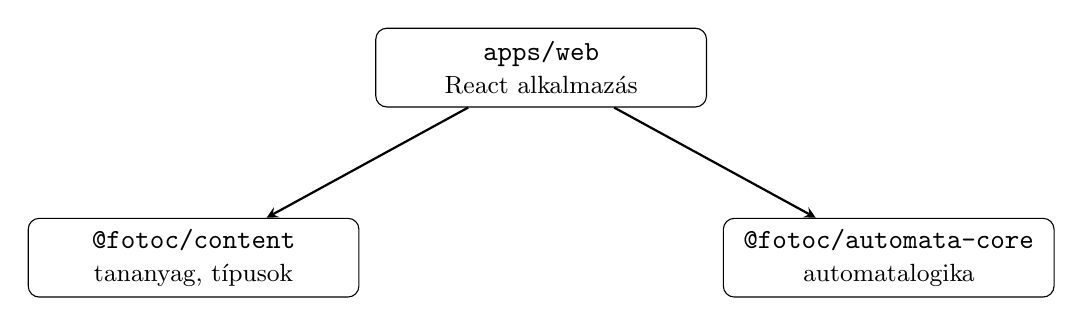
\begin{tikzpicture}[
        pkg/.style={draw, rounded corners, minimum width=4.2cm,
                    minimum height=1cm, align=center},
        dep/.style={-stealth, thick}
    ]
        \node[pkg] (web) {\texttt{apps/web}\\\small React alkalmazás};
        \node[pkg, below left=1.4cm and 0.2cm of web] (content)
            {\texttt{@fotoc/content}\\\small tananyag, típusok};
        \node[pkg, below right=1.4cm and 0.2cm of web] (core)
            {\texttt{@fotoc/automata-core}\\\small automatalogika};
        \draw[dep] (web) -- (content);
        \draw[dep] (web) -- (core);
    \end{tikzpicture}
    \caption{A csomagok közötti függőségek}
    \label{fig:packages}
\end{figure}

\section{A tartalomcsomag (\texttt{@fotoc/content})}

A csomag a~\ref{sec:data}.~szakaszban leírt típusokat és a
témakörök adatait tartalmazza. Minden témakör saját mappát kap
két fájllal: a \texttt{meta.ts} a metaadatokat, a \texttt{theory.ts}
az elméleti anyag blokkjait exportálja.

A témakörök összegyűjtését a \texttt{topics/index.ts} végzi
(\emph{topic registry}). Ez importálja az összes témakört, a
\texttt{order} mező szerint rendezi őket, és a csomag két belépési
pontot ad a webalkalmazásnak:

\begin{itemize}
    \item \texttt{topics}: az összes témakör rendezett listája;
    \item \texttt{getTopic(id)}: egy témakör lekérése azonosító alapján
          (\texttt{undefined}, ha nem létezik).
\end{itemize}

A registry jelenleg kézzel karbantartott lista, ami a prototípus
szakaszban egyszerű és átlátható megoldás. Egy új témakör felvétele
tehát három lépésből áll: új mappa \texttt{meta.ts} és
\texttt{theory.ts} fájllal, majd a két import és a bejegyzés felvétele
az \texttt{index.ts}-be. Később ez a Vite \texttt{import.meta.glob}
funkciójával automatizálható.

\section{A webalkalmazás (\texttt{apps/web})}

\subsection{Útvonalak}

Az alkalmazás a React Router segítségével két oldalt szolgál ki:

\begin{table}[htbp]
    \centering
    \begin{tabularx}{\textwidth}{l l X}
        \toprule
        \textbf{Útvonal} & \textbf{Komponens} & \textbf{Feladat} \\
        \midrule
        \texttt{/}                  & \texttt{Homepage}   &
            Az összes témakör listázása, mindegyik hivatkozással a saját
            oldalára. \\
        \texttt{/topics/:topicID}   & \texttt{Topicpages} &
            Egy témakör címének, összefoglalójának, csoportjának, a
            kapcsolódó előadásoknak és az elméleti anyagnak a
            megjelenítése. \\
        \bottomrule
    \end{tabularx}
    \caption{Az alkalmazás útvonalai}
    \label{tab:routes}
\end{table}

A témakör oldala az URL-ből kapott azonosítóval hívja meg a
\texttt{getTopic} függvényt. Ha ilyen azonosítójú témakör nincs,
hibaüzenetet jelenít meg.

\subsection{Az elméleti anyag megjelenítése}

Az elméleti blokkokat a \texttt{TheoryRenderer} komponens rajzolja ki.
A komponens végigmegy a témakör blokkjain, és mindegyikhez a
\texttt{type} mező alapján választja ki a megfelelő HTML-elemet. Mivel
a \texttt{ContentBlock} diszkriminált unió, a TypeScript az egyes
ágakban tudja, milyen mezői vannak az adott blokknak (például a
\texttt{heading} ágban elérhető a \texttt{level} mező, a
\texttt{formula} ágban a \texttt{latex}). Egy új blokktípus
bevezetésekor így elég a típust és a megjelenítő egy új ágát megírni.

% Frissíteni, ahogy halad a renderer.
Jelenleg a címsor és a bekezdés blokkok megjelenítése készült el, a
többi blokktípus kirajzolása és a képletek KaTeX-alapú megjelenítése
a következő fejlesztési lépés.

\section{Az automatacsomag (\texttt{@fotoc/automata-core})}

Ez a csomag fogja tartalmazni az automaták és algoritmusok
megjelenítéstől független logikáját (például egy DVA lépésenkénti
futtatását egy bemeneti szón). A csomag szerkezete és a webalkalmazással
való kapcsolata már kialakításra került, a tényleges implementáció a
szimulációs modul fejlesztésével együtt készül el.

\begin{thebibliography}{9}
    \bibitem{icons}
        seanyasno: \emph{Handling icons in React: best practices}. DEV Community.
        \url{https://dev.to/seanyasno/handling-icons-in-react-best-practices-22c5}
\end{thebibliography}

\end{document}
